\documentclass[tikz,border=6pt]{standalone}

\usepackage[T1]{fontenc}
\usepackage[utf8]{inputenc}
\usepackage{lmodern}
\usepackage{tikz}
\usepackage{xcolor}
\usetikzlibrary{arrows.meta,positioning,calc}

\begin{document}

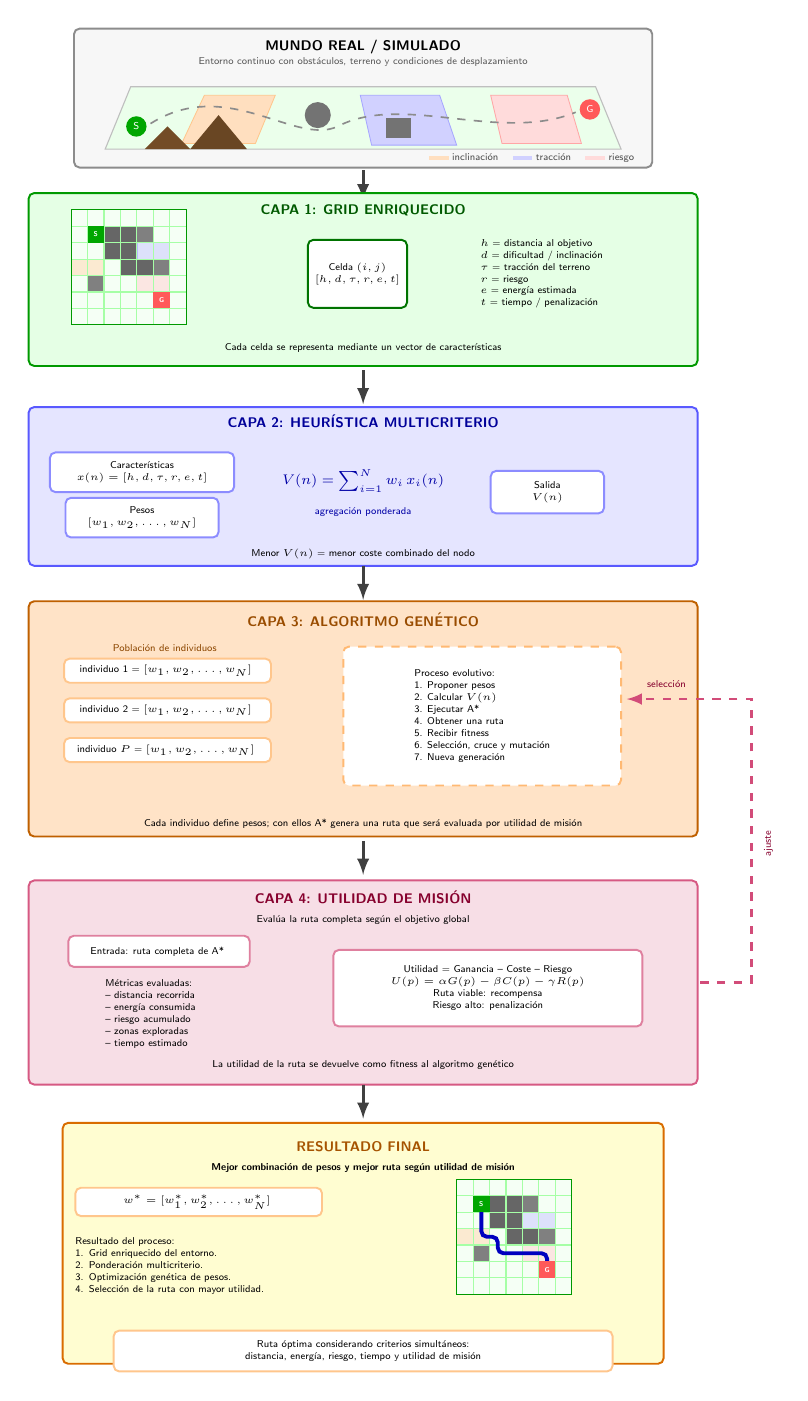
\begin{tikzpicture}[
  scale=0.72,
  transform shape,
  font=\sffamily,
  box/.style={rounded corners=2pt, line width=0.7pt, align=center},
  small/.style={font=\sffamily\scriptsize},
  tinytxt/.style={font=\sffamily\tiny},
  celllabel/.style={font=\sffamily\bfseries\large},
  arrow/.style={-latex, line width=1pt, draw=black!75},
  feedback/.style={-latex, dashed, line width=0.9pt, draw=purple!70}
]

% -------------------------------------------------
% TÍTULO
% -------------------------------------------------
% Arquitectura por capas para planificación de rutas con heurística multicriterio,
% algoritmo genético y utilidad de misión
% convertir en pdf: pdflatex figura_arquitectura_standalone.tex

% -------------------------------------------------
% MUNDO REAL / SIMULADO
% -------------------------------------------------
\node[
  box,
  draw=black!45,
  fill=gray!6,
  minimum width=10.2cm,
  minimum height=2.45cm
] (world) at (0,-1.95) {};

\node[
  small,
  font=\sffamily\scriptsize\bfseries
] at (0,-1.05) {
MUNDO REAL / SIMULADO
};

\node[
  tinytxt,
  text=black!65
] at (0,-1.32) {
Entorno continuo con obstáculos, terreno y condiciones de desplazamiento
};

% Superficie base / terreno
\draw[
  fill=green!8,
  draw=black!25,
  line width=0.4pt
] (-4.55,-2.85) -- (4.55,-2.85) -- (4.1,-1.75) -- (-4.1,-1.75) -- cycle;

% Zonas de dificultad del terreno
\fill[orange!25, draw=orange!45, line width=0.3pt]
  (-3.2,-2.75) -- (-1.9,-2.75) -- (-1.55,-1.9) -- (-2.8,-1.9) -- cycle;

\fill[blue!18, draw=blue!35, line width=0.3pt]
  (0.15,-2.78) -- (1.65,-2.78) -- (1.35,-1.9) -- (-0.05,-1.9) -- cycle;

\fill[red!14, draw=red!35, line width=0.3pt]
  (2.45,-2.75) -- (3.85,-2.75) -- (3.6,-1.9) -- (2.25,-1.9) -- cycle;

% Obstáculos
\fill[black!55] (-0.8,-2.25) circle (0.23);
\fill[black!55] (0.40,-2.65) rectangle ++(0.45,0.35);

% Relieve / pendientes
\fill[brown!60!black]
  (-3.45,-2.45) -- (-3.85,-2.85) -- (-3.05,-2.85) -- cycle;

\fill[brown!55!black]
  (-2.55,-2.25) -- (-3.05,-2.85) -- (-2.05,-2.85) -- cycle;

% Inicio y objetivo
\fill[green!65!black] (-4.0,-2.45) circle (0.18);
\node[tinytxt, white] at (-4.0,-2.45) {S};

\fill[red!65] (4.0,-2.15) circle (0.18);
\node[tinytxt, white] at (4.0,-2.15) {G};

% Trayectoria conceptual discontinua, no ruta calculada
\draw[
  dashed,
  line width=0.6pt,
  draw=black!45
]
(-3.75,-2.4)
  .. controls (-2.4,-1.55) and (-1.2,-2.8) .. (-0.45,-2.45)
  .. controls (0.7,-1.85) and (2.4,-2.75) .. (3.75,-2.2);

% Mini-leyenda interna
\node[
  tinytxt,
  align=left,
  text=black!70
] at (3.0,-3) {
\textcolor{orange!25}{\rule{0.35cm}{0.08cm}} inclinación \quad
\textcolor{blue!18}{\rule{0.35cm}{0.08cm}} tracción \quad
\textcolor{red!14}{\rule{0.35cm}{0.08cm}} riesgo
};

% Flecha hacia Capa 1
\draw[arrow] (0,-3.22) -- (0,-3.75);

% -------------------------------------------------
% CAPA 1: GRID ENRIQUECIDO
% -------------------------------------------------
\node[
  box,
  draw=green!60!black,
  fill=green!10,
  minimum width=11.8cm,
  minimum height=3.05cm
] (c1) at (0,-5.15) {};

\node[
  small,
  text=green!35!black,
  font=\sffamily\scriptsize\bfseries
] at (0,-3.93) {
CAPA 1: GRID ENRIQUECIDO
};

% Grid inicial: mismo entorno que el resultado final, pero sin ruta
\begin{scope}[shift={(-5.15,-5.95)}, scale=0.29]

  % Fondo y grid
  \fill[green!4] (0,0) rectangle (7,7);
  \draw[step=1, green!35] (0,0) grid (7,7);

  % Inicio
  \fill[green!65!black] (1,5) rectangle (2,6);
  \node[celllabel, white] at (1.5,5.5) {S};

  % Objetivo
  \fill[red!65] (5,1) rectangle (6,2);
  \node[celllabel, white] at (5.5,1.5) {G};

  % Obstáculos principales: barrera real que obliga a rodear
  \foreach \x/\y in {
    2/5, 3/5,
    2/4, 3/4,
    3/3, 4/3
  }{
    \fill[black!60] (\x,\y) rectangle +(1,1);
  }

  % Obstáculos secundarios
  \foreach \x/\y in {
    1/2,
    4/5,
    5/3
  }{
    \fill[black!50] (\x,\y) rectangle +(1,1);
  }

  % Zonas ambientales: coste añadido, no obstáculo
  \fill[orange!25,draw=orange!45, line width=0.3pt, opacity=0.65] (0,3) rectangle (2,4); % dificultad / inclinación
  \fill[blue!18, draw=blue!35, line width=0.3pt, opacity=0.65] (4,4) rectangle (6,5);   % tracción / terreno
  \fill[red!15, opacity=0.65] (4,2) rectangle (6,3);                                      % riesgo moderado

  % Redibujar grid encima de zonas ambientales
  \draw[step=1, green!35] (0,0) grid (7,7);

  % Redibujar S y G para que queden visibles
  \fill[green!65!black] (1,5) rectangle (2,6);
  \node[celllabel, white] at (1.5,5.5) {S};

  \fill[red!65] (5,1) rectangle (6,2);
  \node[celllabel, white] at (5.5,1.5) {G};

  % Borde exterior
  \draw[green!60!black, line width=0.45pt] (0,0) rectangle (7,7);

\end{scope}

% Celda enriquecida
\node[
  box,
  draw=green!45!black,
  fill=white,
  minimum width=1.75cm,
  minimum height=1.2cm,
  tinytxt
] at (-0.1,-5.05) {
Celda $(i,j)$\\
$[h,d,\tau,r,e,t]$
};

\node[tinytxt, align=left] at (3.15,-5.05) {
$h$ = distancia al objetivo\\
$d$ = dificultad / inclinación\\
$\tau$ = tracción del terreno\\
$r$ = riesgo\\
$e$ = energía estimada\\
$t$ = tiempo / penalización
};

\node[tinytxt] at (0,-6.35) {
Cada celda se representa mediante un vector de características
};

\draw[arrow] (0,-6.75) -- (0,-7.35);

% -------------------------------------------------
% CAPA 2: HEURÍSTICA MULTICRITERIO
% -------------------------------------------------
\node[
  box,
  draw=blue!65,
  fill=blue!10,
  minimum width=11.8cm,
  minimum height=2.8cm
] (c2) at (0,-8.8) {};

\node[
  small,
  text=blue!60!black,
  font=\sffamily\scriptsize\bfseries
] at (0,-7.65) {
CAPA 2: HEURÍSTICA MULTICRITERIO
};

\node[
  box,
  draw=blue!45,
  fill=white,
  minimum width=3.25cm,
  minimum height=0.7cm,
  tinytxt
] at (-3.9,-8.55) {
Características\\
$x(n)=[h,d,\tau,r,e,t]$
};

\node[
  box,
  draw=blue!45,
  fill=white,
  minimum width=2.7cm,
  minimum height=0.7cm,
  tinytxt
] at (-3.9,-9.35) {
Pesos\\
$[w_1,w_2,\ldots,w_N]$
};

\node[small, text=blue!65!black] at (0,-8.7) {
$V(n)=\sum_{i=1}^{N} w_i\,x_i(n)$
};

\node[tinytxt, text=blue!65!black] at (0,-9.25) {
agregación ponderada
};

\node[
  box,
  draw=blue!45,
  fill=white,
  minimum width=2cm,
  minimum height=0.75cm,
  tinytxt
] at (3.25,-8.9) {
Salida\\
$V(n)$
};

\node[tinytxt] at (0,-10.0) {
Menor $V(n)$ = menor coste combinado del nodo
};

\draw[arrow] (0,-10.2) -- (0,-10.8);

% -------------------------------------------------
% CAPA 3: ALGORITMO GENÉTICO
% -------------------------------------------------
\node[
  box,
  draw=orange!75!black,
  fill=orange!22,
  minimum width=11.8cm,
  minimum height=4.15cm
] (c3) at (0,-12.9) {};

\node[
  small,
  text=orange!60!black,
  font=\sffamily\scriptsize\bfseries
] at (0,-11.15) {
CAPA 3: ALGORITMO GENÉTICO
};

\node[tinytxt, text=orange!55!black] at (-3.5,-11.65) {
Población de individuos
};

\node[
  box,
  draw=orange!45,
  fill=white,
  minimum width=3.65cm,
  minimum height=0.42cm,
  tinytxt
] at (-3.45,-12.05) {
individuo 1 = $[w_1,w_2,\ldots,w_N]$
};

\node[
  box,
  draw=orange!45,
  fill=white,
  minimum width=3.65cm,
  minimum height=0.42cm,
  tinytxt
] at (-3.45,-12.75) {
individuo 2 = $[w_1,w_2,\ldots,w_N]$
};

\node[
  box,
  draw=orange!45,
  fill=white,
  minimum width=3.65cm,
  minimum height=0.42cm,
  tinytxt
] at (-3.45,-13.45) {
individuo $P$ = $[w_1,w_2,\ldots,w_N]$
};

% Proceso evolutivo
\node[
  box,
  draw=orange!55,
  dashed,
  fill=white,
  minimum width=4.9cm,
  minimum height=2.45cm,
  tinytxt,
  align=left
] at (2.1,-12.85) {
Proceso evolutivo:\\
1. Proponer pesos\\
2. Calcular $V(n)$\\
3. Ejecutar A*\\
4. Obtener una ruta\\
5. Recibir fitness\\
6. Selección, cruce y mutación\\
7. Nueva generación
};

\node[tinytxt] at (0,-14.75) {
Cada individuo define pesos; con ellos A* genera una ruta que será evaluada por utilidad de misión
};

\draw[arrow] (0,-15.05) -- (0,-15.65);

% -------------------------------------------------
% CAPA 4: UTILIDAD DE MISIÓN
% -------------------------------------------------
\node[
  box,
  draw=purple!65,
  fill=purple!13,
  minimum width=11.8cm,
  minimum height=3.6cm
] (c4) at (0,-17.55) {};

\node[
  small,
  text=purple!70!black,
  font=\sffamily\scriptsize\bfseries
] at (0,-16.05) {
CAPA 4: UTILIDAD DE MISIÓN
};

\node[tinytxt] at (0,-16.45) {
Evalúa la ruta completa según el objetivo global
};

\node[
  box,
  draw=purple!50,
  fill=white,
  minimum width=3.2cm,
  minimum height=0.55cm,
  tinytxt
] at (-3.6,-17.0) {
Entrada: ruta completa de A*
};

\node[tinytxt, align=left] at (-3.75,-18.1) {
Métricas evaluadas:\\
-- distancia recorrida\\
-- energía consumida\\
-- riesgo acumulado\\
-- zonas exploradas\\
-- tiempo estimado
};

\node[
  box,
  draw=purple!50,
  fill=white,
  minimum width=5.45cm,
  minimum height=1.35cm,
  tinytxt
] at (2.2,-17.65) {
Utilidad = Ganancia -- Coste -- Riesgo\\
$U(p)=\alpha G(p)-\beta C(p)-\gamma R(p)$\\
Ruta viable: recompensa\\
Riesgo alto: penalización
};

\node[tinytxt] at (0,-19.0) {
La utilidad de la ruta se devuelve como fitness al algoritmo genético
};

% Flecha de feedback: Capa 4 -> Capa 3
\draw[feedback]
  (5.95,-17.55) -- (6.85,-17.55) -- (6.85,-12.55) -- (4.65,-12.55);

\node[tinytxt, text=purple!70!black, rotate=90] at (7.15,-15.1) {
ajuste
};

\node[tinytxt, text=purple!70!black] at (5.35,-12.28) {
selección
};

\draw[arrow] (0,-19.35) -- (0,-19.95);

% -------------------------------------------------
% RESULTADO FINAL
% -------------------------------------------------
\node[
  box,
  draw=orange!85!black,
  fill=yellow!18,
  minimum width=10.6cm,
  minimum height=4.25cm
] (res) at (0,-22.15) {};

\node[
  small,
  text=orange!65!black,
  font=\sffamily\scriptsize\bfseries
] at (0,-20.45) {
RESULTADO FINAL
};

\node[tinytxt, font=\sffamily\tiny\bfseries] at (0,-20.82) {
Mejor combinación de pesos y mejor ruta según utilidad de misión
};

\node[
  box,
  draw=orange!45,
  fill=white,
  minimum width=4.35cm,
  minimum height=0.5cm,
  tinytxt
] at (-2.9,-21.42) {
$w^*=[w_1^*,w_2^*,\ldots,w_N^*]$
};

\node[tinytxt, align=left, text width=4.45cm] at (-2.85,-22.55) {
Resultado del proceso:\\
1. Grid enriquecido del entorno.\\
2. Ponderación multicriterio.\\
3. Optimización genética de pesos.\\
4. Selección de la ruta con mayor utilidad.
};

% Grid final con solución de ruta
\begin{scope}[shift={(1.65,-23.05)}, scale=0.29]

  % Fondo y grid
  \fill[green!4] (0,0) rectangle (7,7);
  \draw[step=1, green!35] (0,0) grid (7,7);

  % Inicio
  \fill[green!65!black] (1,5) rectangle (2,6);
  \node[celllabel, white] at (1.5,5.5) {S};

  % Objetivo
  \fill[red!65] (5,1) rectangle (6,2);
  \node[celllabel, white] at (5.5,1.5) {G};

  % Obstáculos principales
  \foreach \x/\y in {
    2/5, 3/5,
    2/4, 3/4,
    3/3, 4/3
  }{
    \fill[black!60] (\x,\y) rectangle +(1,1);
  }

  % Obstáculos secundarios
  \foreach \x/\y in {
    1/2,
    4/5,
    5/3
  }{
    \fill[black!50] (\x,\y) rectangle +(1,1);
  }

  % Zonas ambientales
  \fill[orange!25, opacity=0.65] (0,3) rectangle (2,4); % dificultad / inclinación
  \fill[blue!18, opacity=0.65] (4,4) rectangle (6,5);   % tracción / terreno
  \fill[red!15, opacity=0.65] (4,2) rectangle (6,3);    % riesgo moderado

  % Redibujar grid encima
  \draw[step=1, green!35] (0,0) grid (7,7);

  % Ruta final calculada
  \draw[
    blue!75!black,
    line width=1.4pt,
    rounded corners=2pt
  ]
    (1.5,5.5)
    -- (1.5,4.5)
    -- (1.5,3.5)
    -- (2.5,3.5)
    -- (2.5,2.5)
    -- (3.5,2.5)
    -- (4.5,2.5)
    -- (5.5,2.5)
    -- (5.5,1.5);

  % Redibujar S y G por encima de la ruta
  \fill[green!65!black] (1,5) rectangle (2,6);
  \node[celllabel, white] at (1.5,5.5) {S};

  \fill[red!65] (5,1) rectangle (6,2);
  \node[celllabel, white] at (5.5,1.5) {G};

  % Borde exterior
  \draw[green!60!black, line width=0.45pt] (0,0) rectangle (7,7);

\end{scope}

\node[
  box,
  draw=orange!45,
  fill=white,
  minimum width=8.8cm,
  minimum height=0.72cm,
  tinytxt
] at (0,-24.05) {
Ruta óptima considerando criterios simultáneos:\\
distancia, energía, riesgo, tiempo y utilidad de misión
};

\end{tikzpicture}

\end{document}